Nesta dissertação foram também desenvolvidos os mecanismos de \textit{deployment} necessários tanto para a versão sem \textit{Kong} bem como para a versão com \textit{Kong}. Neste capítulo é feita uma descrição dos passos necessários para realizar o \textit{deployment}.

%TODO
TODO

\section{Versão sem \textit{Kong}}\label{sec:deployNoKong}

\subsection{Primeira instalação}\label{sec:inst-prim}

Um dos primeiros passos é verificar se na máquina de instalação já se encontra presente o \texttt{git}, o \texttt{docker} e o \texttt{docker-compose}. Caso contrário deve então proceder à sua instalação. A especificação do \texttt{docker-compose} usada é a versão 3.5 pelo que é necessário pelo menos a versão 17.06.0 ou maior do \texttt{docker} e a versão 1.18.0 ou maior do \texttt{docker-compose}. Numa máquina \textit{Ubuntu} pode ser instalado através de~\cite{installDocker,installDC}:
\begin{verbatim}
    sudo apt-get update

    sudo apt-get install git

    sudo apt-get install -y \
        apt-transport-https \
        ca-certificates \
        curl \
        gnupg-agent \
        software-properties-common
    curl -fsSL https://download.docker.com/linux/ubuntu/gpg | sudo apt-key add -
    sudo add-apt-repository \
        "deb [arch=amd64] https://download.docker.com/linux/ubuntu \
        $(lsb_release -cs) \
        stable"
    sudo apt-get update
    sudo apt-get install docker-ce docker-ce-cli containerd.io

    sudo curl -L "https://github.com/docker/compose/releases/download/1.25.5/docker-compose-$(uname -s)-$(uname -m)" -o /usr/local/bin/docker-compose
    sudo chmod +x /usr/local/bin/docker-compose
    sudo ln -s /usr/local/bin/docker-compose /usr/bin/docker-compose
\end{verbatim}

O passo seguinte é abrir as portas na máquina de instalação que serão usadas para a \acrshort{api} dados e/ou interface (É necessário abrir duas portas para a \acrshort{api} de dados (uma {http} e outra \acrshort{https}) e duas para a interface (uma \acrshort{http} e outra \acrshort{https}). Se instalar a \acrshort{api} de dados e a interface na mesma máquina as 4 portas tem de ser diferentes.

Após a instalação das dependências e a abertura das portas necessárias realiza-se a clonagem dos repositórios \texttt{git} que se pretende instalar:
\begin{verbatim}
    git clone https://github.com/jcramalho/CLAV2018.git #para a API de dados
    git clone https://github.com/jcramalho/CLAV2019.git #para a interface
\end{verbatim}

De seguida muda-se para a raiz da pasta da API de dados (\verb|cd CLAV2018|) ou da pasta da interface (\verb|cd CLAV2019|) por forma a seguir mudar para o \textit{branch} \texttt{https} através do comando:

\begin{verbatim}
    git checkout https
\end{verbatim}

Numa versão de produção, é de extrema importância realizar ainda os seguintes passos referentes à configuração da autenticação da \acrshort{clav} (tanto na \acrshort{api} de dados como na interface):
\begin{itemize}
    \item Na \acrshort{api} de dados gerar dois pares de chaves pública/privada:
    \begin{verbatim}
    #assumindo que se encontra na raiz da pasta da API de dados
    openssl genrsa -out config/keys/apiKey 2048
    openssl rsa -in config/keys/apiKey -pubout -out config/keys/apiKey.pub
    openssl genrsa -out config/keys/userKey 2048
    openssl rsa -in config/keys/userKey -pubout -out config/keys/userKey.pub
    \end{verbatim}
    \item Na interface copiar para esta as chaves públicas geradas (este comando apenas funciona se a \acrshort{api} e a interface estão na mesma máquina):
    \begin{verbatim}
    #assumindo que se encontra na raiz da pasta da API de dados
    cp config/keys/apiKey.pub config/keys/userKey.pub \
        <raíz da pasta da interface>/src/plugins/keys/
    \end{verbatim}
\end{itemize}
Sem a realização destes passos qualquer utilizador que consiga saber as chaves privadas usadas (por exemplo através do \textit{GitHub}) pode gerar um \textit{token} e assim ter acesso indevido à \acrshort{clav}. Portanto as chaves privadas devem estar apenas acessíveis na máquina de produção da \acrshort{api} de dados (não partilhe nem faça \textit{push} destas chaves).

Antes de se realizar os próximos passos, faz-se ainda uma última mudança de raiz para a pasta \texttt{deploy} (\verb|cd deploy|). Nesta raiz é onde será realizado os passos seguintes das próximas secções.
\subsubsection{Criação de Imagens}

As imagens usadas na instalação podem ser geradas com antecedência, fora da máquina de instalação. Para isso essas imagens geradas devem ser registadas no (\textit{push} para o) \textit{DockerHub} para posterior uso.

\begin{description}
    \item \textbf{\acrshort{api} de dados}

    Necessário realizar a criação de duas imagens: \texttt{graphdb} e \texttt{server}.

    Para criar a imagem \texttt{graphdb} é necessário dois ficheiros adicionais: um ficheiro zip com a distribuição do \textit{GraphDB} e um ficheiro \textit{Turtle} com a ontologia a carregar para o \textit{GraphDB}. A distribuição do \textit{GraphDB} deve ser obtida através do site \textit{GraphDB}\footnote{Versão gratuita: \url{https://www.ontotext.com/products/graphdb/graphdb-free/}} ao preencher o formulário. Após o preenchimento do formulário irá receber um email do \textit{GraphDB}. Nesse email deve realizar \textit{download} da versão ``stand-alone server'' ao carregar no \textit{link} ``Download as a stand-alone server''. O ficheiro zip tem um nome parecido com ``graphdb-free-8.11.0-dist.zip''. A zona ``free-8.11.0'' indica a versão do \textit{GraphDB} que deve colocar na variável ambiente \texttt{GRAPHDB\_VERSION} do ficheiro .env da pasta \texttt{deploy}. Deve colocar o ficheiro zip na pasta \texttt{graphdb} da pasta \texttt{deploy}. Nesta pasta (\texttt{graphdb}) deve também colocar o ficheiro \textit{Turtle} e indicar na variável ambiente \texttt{GRAPHDB\_DATA\_FILE} o nome deste ficheiro (ex: clav-2020-01-04-false.ttl). Sempre que um destes ficheiros é alterado é necessário criar de novo a imagem.

    \begin{figure}[H]
        \begin{center}
        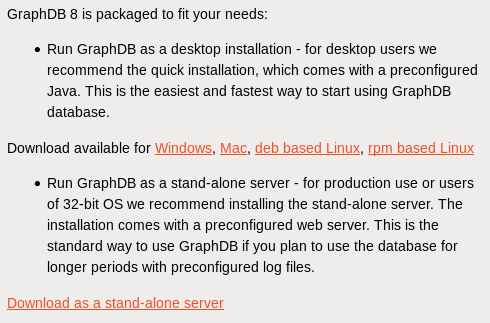
\includegraphics[width=0.4\textwidth]{img/graphdb_email.png}
        \end{center}
        \caption{Parte do email recebido pelo GraphDB\label{fig:instalacao-email}}
    \end{figure}

    A criação de uma nova imagem \texttt{server} é apenas necessária na primeira instalação e quando o código da \acrshort{api} de dados muda.

    \item \textbf{Interface}

    Existe apenas uma imagem (\texttt{interface}) que deve ser recriada sempre que a versão da \acrshort{api} de dados (variável ambiente \texttt{API\_VERSION} do ficheiro .env da pasta \textit{deploy}) ou o \acrshort{url} da \acrshort{api} de dados (variável ambiente \texttt{API\_URL} do ficheiro .env da pasta \textit{deploy}) ou o código mude.
\end{description}

Agora, através do ficheiro \textit{docker-compose-build.yaml} é possível criar as imagens. Pode associar uma \textit{tag} a cada imagem a criar, no ficheiro \textit{.env} da \acrshort{api} de dados, nas variáveis ambiente \texttt{GRAPHDB\_IMG} (imagem \texttt{graphdb}) e \texttt{SERVER\_IMG} (imagem \texttt{server}) onde deve inserir o nome do repositório do \textit{DockerHub} e a \textit{tag} a usar (\verb|<repositório>:<tag>|, ex: jcm300/clav\_api:1.0.0). Já no ficheiro \textit{.env} da interface está presente a variável ambiente \texttt{INTERFACE\_IMG} com o mesmo intuito mas para a imagem da interface. Para criar estas imagens basta correr na pasta \texttt{deploy} da \acrshort{api} de dados (para criar as imagens da \acrshort{api} de dados) ou da interface (para criar a imagem da interface):

\begin{verbatim}
    docker-compose -f docker-compose-build.yml build
\end{verbatim}

Para criar apenas uma das imagens indique à frente o nome do serviço:
\begin{verbatim}
    docker-compose -f docker-compose-build.yml build <nome do serviço (ex: server)>
\end{verbatim}

Depois de criadas as imagens se pretender torná-las disponíveis no \textit{DockerHub} deve para cada uma delas realizar o seguinte comando:
\begin{verbatim}
    docker push <repositório>:<tag>
\end{verbatim}
O comando pode falhar por duas razões. A primeira pelo facto de o utilizador ainda não se ter autenticado com a sua conta do \textit{DockerHub} através do comando \verb|docker login|. A segunda é pelo facto de que o repositório para o qual pretende fazer push da imagem não se encontra criado no \textit{DockerHub}. Nesse caso deve aceder o site do \textit{DokerHub} e criar o repositório.

\subsubsection{Configuração}\label{sec:int-config}
Tanto na \acrshort{api} de dados como na interface na pasta \texttt{deploy} está presente um ficheiro \textit{.env} já referido várias vezes nas secções anteriores. Estes ficheiros permitem configurar respetivamente a instalação da \acrshort{api} de dados e da interface.

Na \acrshort{api} de dados para além das já referidas variáveis ambiente (\texttt{GRAPHDB\_VERSION}, \texttt{GRAPHDB\_DATA\_FILE}, \texttt{GRAPHDB\_IMG} e \texttt{SERVER\_IMG}) possui também as seguintes variáveis ambiente:
\begin{itemize}
    \item \texttt{CERT\_FOLDER}: Pasta onde estão os ficheiros do certificado no \textit{container} \texttt{nginx}
    \item \texttt{ACME\_FOLDER}: Pasta onde estão os ficheiros do \texttt{acme.sh} no \textit{container} \texttt{nginx}
    \item \texttt{API\_VERSION}: Versão da \acrshort{api} de dados
    \item \texttt{DOMAINS}: Domínios dos quais a \acrshort{api} de dados irá estar acessível
    \item \texttt{SWAGGER\_URL}: \acrshort{url} principal a colocar na documentação \textit{OpenAPI} (\textit{Swagger})
    \item \texttt{INTERFACE\_HOSTS}: \textit{Hosts} nos quais há interfaces da CLAV
    \item \texttt{HTTP\_PORT}: Porta \acrshort{http} em que a \acrshort{api} de dados recebe os pedidos \acrshort{http} dentro da máquina de instalação
    \item \texttt{HTTPS\_PORT}: Porta \acrshort{https} em que a \acrshort{api} de dados recebe os pedidos \acrshort{https} dentro da máquina de instalação
\end{itemize}
Caso estas variáveis ambiente sejam alteradas não implica recriar as imagens mas sim apenas reiniciar os \textit{containers}.

Quanto à interface para além das já referidas variáveis ambiente (\texttt{API\_VERSION}, \texttt{API\_URL} e \texttt{INTERFACE\_IMG}) possui também as seguintes variáveis ambiente:
\begin{itemize}
    \item \texttt{CERT\_FOLDER}: Pasta onde estão os ficheiros do certificado no \textit{container} \texttt{interface}
    \item \texttt{ACME\_FOLDER}: Pasta onde estão os ficheiros do \texttt{acme.sh} no \textit{container} \texttt{interface}
    \item \texttt{DOMAINS}: Domínios dos quais a interface irá estar acessível
    \item \texttt{SERVER\_URL}: \acrshort{url} da \acrshort{api} de dados
    \item \texttt{HTTP\_PORT}: Porta \acrshort{http} em que a interface recebe os pedidos \acrshort{http} dentro da máquina de instalação
    \item \texttt{HTTPS\_PORT}: Porta \acrshort{https} em que a interface recebe os pedidos \acrshort{https} dentro da máquina de instalação   
    \item \texttt{NGINX\_FILE}: Ficheiro de configuração \textit{Nginx} a usar. Duas hipóteses:
    \begin{itemize}
        \item \texttt{nginx.conf.template}: A interface não faz redirecionamento dos pedidos que recebe para a \acrshort{api} de dados. O valor de \texttt{API\_URL} tem de ser o \acrshort{url} real da \acrshort{api} de dados (será igual a \texttt{SERVER\_URL})
        \item \texttt{nginxProxy.conf.template}: A interface faz redirecionamento dos pedidos que recebe para a \acrshort{api} de dados. O valor de \texttt{API\_URL} tem de ser o \acrshort{url} da interface, estando em \texttt{SERVER\_URL} o \acrshort{url} real da \acrshort{api} de dados
    \end{itemize}
\end{itemize}
Caso sejam alteradas estas variáveis ambiente não implica recriar a imagem mas sim apenas reiniciar o \textit{container}.

Após realizar as alterações necessárias pode correr o seguinte comando na pasta \texttt{deploy} da API de dados (para iniciar a API de dados) ou da interface (para iniciar a interface) se as imagens (\texttt{server} e \texttt{graphdb} ou \texttt{interface}) foram criadas localmente ou estejam presentes no \textit{DockerHub} (mude as variáveis ambiente \texttt{GRAPHDB\_IMG} e \texttt{SERVER\_IMG} na \acrshort{api} de dados ou \texttt{INTERFACE\_IMG} na interface para usar as imagens do \textit{DockerHub} que pretende):

\begin{verbatim}
    docker-compose up
\end{verbatim}

Caso as imagens (\texttt{server} e \texttt{graphdb} ou \texttt{interface}) ainda não estejam criadas nem presentes no \textit{DockerHub} pode criá-las e de seguida iniciá-las através do comando:

\begin{verbatim}
    docker-compose -f docker-compose-build.yml up
\end{verbatim}

Pode forçar a criação das imagens (útil visto que por vezes o comando anterior não recria as imagens quando algo é alterado):

\begin{verbatim}
    docker-compose -f docker-compose-build.yml up --build
\end{verbatim}

De seguida refere-se umas notas adicionais de extrema importância quanto aos volumes associados aos \textit{containers} tanto na \acrshort{api} de dados como na interface.

Na \acrshort{api} de dados se pretende manter os dados entre atualizações (criação de novas imagens e reinícios dos \textit{containers}) não deve eliminar os volumes \texttt{clav-mongodb-data} (dados da \acrshort{bd} \textit{MongoDB}) e \texttt{clav-graphdb-data} (dados da \acrshort{bd} \textit{GraphDB}). Além disso, não deve eliminar os volumes \texttt{acme-data} e \texttt{crontabs}, o primeiro para não ser necessário gerar novos certificados (podendo atingir o limite de geração de certificados do \textit{Let's Encrypt}) e o segundo visto ser o ficheiro de configuração que permite que execute periodicamente (diariamente) o \texttt{acme.sh} para verificar se os certificados tem apenas 30 dias de validade e como tal proceder à renovação destes.

Do lado da interface os volumes que não deve eliminar são \texttt{acme-interface-data} e \texttt{crontabs-interface} pelas mesmas razões já referidas antes para os volumes \texttt{acme-data} e \texttt{crontabs}. 

\subsubsection{Povoamento do MongoDB}
Até ao momento neste procedimento de instalação a \acrshort{bd} \textit{MongoDB} continua vazia. Se já possui uma \acrshort{bd} do \textit{MongoDB} já povoada é possível proceder à migração. Caso contrário precisará de pelo menos inserir à mão (através do cliente do \textit{MongoDB}) um utilizador com o nível de Administrador de Perfil Tecnológico à coleção \texttt{users}.

\begin{description}
    \item \textbf{Backup}

    De forma a realizar a migração é necessário primeiro fazer o backup da \acrshort{bd} já povoada. Caso possua apenas uma \acrshort{bd} no \textit{MongoDB} o backup pode ser efetuado através de:

    \begin{verbatim}
    F=$(pwd) && cd <caminho da BD do MongoDB> && tar -cvf $F/backup.tar . && cd $F
    \end{verbatim}

    O caminho \textit{default} da \acrshort{bd} do \textit{MongoDB} pode ser \path{/var/lib/mongodb} ou \path{/data/db} em sistemas \textit{Unix}.
    Já, caso possua várias bases de dados no mesmo caminho recomenda-se então realizar o seguinte comando de forma a realizar backup:

    \begin{verbatim}
    mongodump --db <nome da BD> --out <caminho a guardar o backup>
    \end{verbatim}

    No destino final será criada uma pasta com o nome da \acrshort{bd} que irá possuir o backup da \acrshort{bd}.
    De forma a realizar o backup através do \texttt{mongodump} é necessário que o \textit{MongoDB} esteja a correr.

    \item \textbf{Inserção}

    Primeiro pare os containers:
    \begin{verbatim}
    docker stop clav_nginx
    docker stop clav_server
    docker stop clav_mongo clav_graphdb
    \end{verbatim}

    A inserção da informação do backup no volume irá depender da forma que foi feita o backup. 

    No primeiro caso, a inserção da informação é obtida através da execução do seguinte comando:
    \begin{verbatim}
    docker run --rm -v clav-mongodb-data:/data/db -v $(pwd):/backup ubuntu \
        bash -c "cd /data/db && tar -xvf /backup/backup.tar"
    \end{verbatim}

    Quanto ao caso em que é realizado o \texttt{mongodump} deve-se executar o seguinte comando:
    \begin{verbatim}
    docker run --rm -v clav-mongodb-data:/data/db \
        -v <caminho absoluto onde foi guardado o backup>/<nome da BD>:/backup mongo \
        bash -c "(mongod &) && mongorestore --db <nome da BD> --drop /backup"
    \end{verbatim}

    Por fim, volte a iniciar os containers:
    \begin{verbatim}
    docker start clav_mongo clav_graphdb
    docker start clav_server
    docker start clav_nginx
    \end{verbatim}
\end{description}

\subsubsection{Melhorias de segurança do HTTPS}
Após concluir a instalação recomenda-se duas melhorias de segurança do \acrshort{https} em que uma delas apenas se pode realizar agora. Nesta secção sempre que se referir o domínio ou domínios pretende-se fazer referência aos presentes nos \texttt{DOMAINS} dos ficheiros de configuração \texttt{.env} da \acrshort{api} de dados e da interface.

A melhoria que apenas se pode realizar agora é a adição dos domínios usados à \textit{\acrshort{hsts} preload list}. Para isso deve aceder a \url{https://hstspreload.org/}, começar por inserir um dos domínios e seguir os passos indicados. Repita para os restantes domínios. 

Esta melhoria é necessária visto que foi configurada a header \acrshort{hsts} que avisa o browser para usar sempre \acrshort{ssl}/\acrshort{tls} para comunicar com o site. Contudo, existe uma vulnerabilidade que acontece na primeira conexão com o domínio. Para tal, existe o \textit{HSTS preloading}. O \textit{HSTS preloading} é nada mais que uma lista pré carregada pelos browsers com os vários domínios em que a header \acrshort{hsts} está definida. Assim o browser logo à partida sabe se o(s) domínio/dominío(s) deve(m) ser acedido(s) apenas por \acrshort{https}. Para tal na header \acrshort{hsts} foi adicionada a keyword \texttt{preload} para depois adicionar os domínios através do link já referido. Se pretender não ativar o \textit{\acrshort{hsts} preloading} ou não for elegível retire a keyword \texttt{preload} da header \acrshort{hsts} nos ficheiros de configuração \textit{Nginx} da \acrshort{api} de dados e/ou da interface.

A outra melhoria de segurança é referente à configuração do \acrshort{dns} no qual os domínios estão indexados. Ao \acrshort{dns} (tem de suportar records \acrshort{caa}) devem ser adicionados records \acrshort{caa} associados aos domínios a usar. Os records \acrshort{caa} a adicionar podem ser obtidos em \url{https://sslmate.com/caa/} indicando o nome do domínio e escolhendo como \textit{Authorized Certificate Authorities} o \textit{Let's Encrypt}. Na secção 4 da página Web é apresentado os records \acrshort{caa}. Repita para os restantes domínios. 

O objetivo destes records \acrshort{caa} é indicar a(s) autoridade(s) emissora(s) de certificados permitida(s) para o(s) domínio(s) por forma a impedir que seja emitido um certificado para o(s) mesmo(s) domínio(s) noutra autoridade emissora de certificados, minimizando o risco de vulnerabilidades de segurança de outros emissores de certificados.

\subsection{Atualizações}

Tal como a instalação, as atualizações podem ser feitas de forma separada, ou seja, é possível atualizar apenas a \acrshort{api} de dados ou apenas a interface ou até as duas se assim o pretender.

Para tal, deve-se primeiro parar os \textit{containers}:
\begin{itemize}
    \item \texttt{clav\_mongo}, \texttt{clav\_graphdb}, \texttt{clav\_server} e \texttt{clav\_nginx} no caso da \acrshort{api} de dados:
    \begin{verbatim}
    docker stop clav_nginx
    docker stop clav_server
    docker stop clav_mongo clav_graphdb
    \end{verbatim}
    \item \texttt{interface} no caso da interface:
    \begin{verbatim}
    docker stop interface
    \end{verbatim}       
\end{itemize}

Antes de recriar as imagens se pretender realizar push destas deve alterar as \textit{tags} nos ficheiros de configuração \texttt{.env} da imagem(s) que precisará de recriar por forma a não sobescrever \textit{tags}. Fica à escolha do utilizador. Apenas tem de ter em conta que as variáveis ambiente \texttt{GRAPHDB\_IMG}, \texttt{SERVER\_IMG} e \texttt{INTERFACE\_IMG} podem ser utilizadas para gerir as imagens da forma que pretender.

De seguida recria-se os \textit{containers} necessários:
\begin{itemize}
    \item Caso tenha mudado a ontologia ou pretenda atualizar a distribuição do \textit{GraphDB} recria-se a imagem do \texttt{clav\_graphdb} após as devidas alterações no ficheiro .env da pasta \textit{deploy}. Comando a executar para recriar:
    \begin{verbatim}
    docker-compose -f docker-compose-build.yml build graphdb
    \end{verbatim}
    \item Caso tenha sido alterado código na \acrshort{api} de dados (\verb|git pull|) recria-se a imagem do \texttt{clav\_server}. Comando a executar para recriar:
    \begin{verbatim}
    git pull #obter novos commits
    docker-compose -f docker-compose-build.yml build server
    \end{verbatim}
    \item Caso tenha sido alterado código da interface (\verb|git pull|) ou uma das variáveis ambientes \texttt{API\_URL} e/ou \texttt{API\_VERSION} tenham sido alteradas recria-se a imagem da \texttt{interface}. Comando a executar para recriar:
    \begin{verbatim}
    git pull #obter novos commits
    docker-compose -f docker-compose-build.yml build interface
    \end{verbatim}
\end{itemize}
Caso no build seja usado a cache para construir as imagens muito provavelmente as imagens criadas serão iguais às já existentes. Nesse caso adicione a \textit{flag} \verb|--no-cache| no comando de build.

Por fim, volta-se a iniciar os \textit{containers} da \acrshort{api} de dados ou da interface dependendo em que pasta \texttt{deploy} está através do comando:
\begin{verbatim}
    docker-compose up
\end{verbatim}

\subsection{Backup}\label{sec:inst-backup}

Em termos de backup, os volumes de maior importância são o do \textit{MongoDB} e o do \textit{GraphDB} visto possuírem toda a informação da \acrshort{clav}. Note que este backup apenas implica a \acrshort{api} de dados. Por forma a realizar o backup deve:
\begin{verbatim}
    #parar containers
    docker stop clav_nginx
    docker stop clav_server
    docker stop clav_mongo clav_graphdb
    
    #backup do volume do GraphDB
    docker run --rm --volumes-from clav_graphdb \
        -v $(pwd):/backup ubuntu \
        bash -c "cd /opt/graphdb/home/data/repositories && \
        tar cvf /backup/clav_graphdb.tar ."
        
    #backup do volume do MongoDB
    docker run --rm --volumes-from clav_mongo \
        -v $(pwd):/backup ubuntu bash -c "cd /data/db && \
        tar cvf /backup/clav_mongo.tar ."
        
    #Pode agora voltar a iniciar os containers
    docker start clav_mongo clav_graphdb
    docker start clav_server
    docker start clav_nginx
\end{verbatim}

No final possuirá dois ficheiros tar (clav\_graphdb.tar e clav\_mongo.tar) na raiz onde executou os comandos que são respetivamente o backup do \textit{GraphDB} e o backup do \textit{MongoDB}.

A partir daqui pode armazenar estes onde achar mais conveniente e seguro.

\subsection{Migração}

Para realizar a migração para outra máquina é necessário primeiro realizar o backup dos volumes da máquina atual. Pode para isso seguir a secção~\ref{sec:inst-backup}. Depois deve copiar os vários ficheiros comprimidos (.tar) para a nova máquina de instalação.

Os passos seguintes serão a realização da primeira instalação na nova máquina, bastando para isso seguir a secção~\ref{sec:inst-prim} mas sem realizar o povoamento do MongoDB.

O passo final é restaurar os volumes através dos backups (ficheiros comprimidos .tar). Para tal siga os seguintes passos para restaurar os volumes:
\begin{verbatim}
    #assumindo que se encontra na raiz onde se encontram os ficheiros tar

    #parar containers
    docker stop clav_nginx
    docker stop clav_server
    docker stop clav_mongo clav_graphdb
    
    #restauro do volume do GraphDB
    docker run --rm -v clav-graphdb-data:/opt/graphdb/home/data/repositories \
        -v $(pwd):/backup ubuntu bash -c "cd /opt/graphdb/home/data/repositories \
        && tar xvf /backup/clav_graphdb.tar"
        
    #restauro do volume do MongoDB
    docker run --rm -v clav-mongodb-data:/data/db \
        -v $(pwd):/backup ubuntu bash -c "cd /data/db \
        && tar xvf /backup/clav_mongo.tar"
        
    #voltar a iniciar os containers
    docker start clav_mongo clav_graphdb
    docker start clav_server
    docker start clav_nginx
\end{verbatim}

Pode também dividir a \acrshort{api} de dados e a interface por duas máquinas. Para isso deve realizar na mesma o backup dos volumes na máquina atual, seguir a primeira instalação individualmente para cada máquina (instalando apenas a componente correspondente), copiar os backups apenas para a máquina da \acrshort{api} de dados e restaurar esses backups.

%TODO
TODO

\section{Versão com \textit{Kong}}\label{sec:deployKong}

%TODO
TODO

\section{Resumo}

%TODO
TODO
